\documentclass[a4paper,12pt]{article}

\usepackage[T2A]{fontenc}			
\usepackage[utf8]{inputenc}			
\usepackage[english,russian]{babel}	

\usepackage[
bookmarks=true, colorlinks=true, unicode=true,
urlcolor=black,linkcolor=black, anchorcolor=black,
citecolor=black, menucolor=black, filecolor=black,
]{hyperref}

\usepackage{color}
\usepackage{caption}
\DeclareCaptionFont{white}{\color{black}}
\DeclareCaptionFormat{listing}{\colorbox{white}{\parbox{\textwidth}{#1#2#3}}}
\captionsetup[lstlisting]{format=listing,labelfont=white,textfont=white}

\usepackage{amsmath,amsfonts,amssymb,amsthm,mathtools} 
\usepackage{wasysym}

\usepackage{graphicx}
%\usepackage[cache=false]{minted}
\usepackage{cmap}
\usepackage{indentfirst}

\usepackage{listings} 
\usepackage{fancyvrb}

\usepackage{geometry}
\geometry{left=2cm}
\geometry{right=1.5cm}
\geometry{top=1cm}
\geometry{bottom=2cm}

\setlength{\parindent}{5ex}
\setlength{\parskip}{0.5em}

\usepackage{pgfplots}
\usetikzlibrary{datavisualization}
\usetikzlibrary{datavisualization.formats.functions}

\begin{document}
	\lstset{ %
		language=C,                 % выбор языка для подсветки (здесь это С)
		basicstyle=\small\sffamily, % размер и начертание шрифта для подсветки кода
		numbers=left,               % где поставить нумерацию строк (слева\справа)
		numberstyle=\tiny,           % размер шрифта для номеров строк
		stepnumber=1,                   % размер шага между двумя номерами строк
		numbersep=5pt,                % как далеко отстоят номера строк от подсвечиваемого кода
		backgroundcolor=\color{white}, % цвет фона подсветки - используем \usepackage{color}
		showspaces=false,            % показывать или нет пробелы специальными отступами
		showstringspaces=false,      % показывать или нет пробелы в строках
		showtabs=false,             % показывать или нет табуляцию в строках
		frame=single,              % рисовать рамку вокруг кода
		tabsize=2,                 % размер табуляции по умолчанию равен 2 пробелам
		captionpos=t,              % позиция заголовка вверху [t] или внизу [b] 
		breaklines=true,           % автоматически переносить строки (да\нет)
		breakatwhitespace=false, % переносить строки только если есть пробел
		escapeinside={\%*}{*)}   % если нужно добавить комментарии в коде
	}
	
	% Титульный лист
	\begin{figure}[h!]
		\begin{center}
			{
\includegraphics[scale = 0.4]{titul.jpg}}
			\label{titul}
		\end{center}
	\end{figure}
	
	\vspace*{15mm} 
	
	\huge
	\begin{center}
		Дисциплина: <<Функциональное и логическое программирование>>
	\end{center}
	\vspace*{15mm} 	
	
	\begin{center}
		Лабораторная работа №12
	\end{center}
	
	\vspace*{15mm} 	
	
	\large
	\begin{flushright}
		Студент: Левушкин И. К. \\
		Группа: ИУ7-62Б \\
		Преподаватели: Толпинская Н. Б., \\ Строганов Ю. В. \\
	\end{flushright}
	
	\vspace*{30mm}
	\begin{center}
		Москва, 2020 г.  
	\end{center}
	\thispagestyle{empty}
	
	
	\newpage
	
	\section{Задание}
	
	Составить программу – базу знаний, с помощью которой можно определить, например, множество студентов, обучающихся в одном ВУЗе. Студент может одновременно обучаться в нескольких ВУЗах. Привести примеры возможных вариантов вопросов и варианты ответов (не менее 3-х). Описать порядок формирования вариантов ответа.
	Исходную базу знаний сформировать с помощью только фактов. 
	*Исходную базу знаний сформировать, используя правила.
	*Разработать свою базу знаний (содержание произвольно).
	
	\section{Реализация программы}
	
	Ниже приведен листинг кода программы - базы знаний, соответствующей поставленной задаче.
	
	\begin{lstlisting}[label = lst0, caption = Листинг кода программы]
	domains
	    student = person(fio, string Phone, birthday).
	    fio = name(string First, string Last).
	    birthday = b_date(string Month, integer Day, integer Year).
	    info = inf(string Faculty, integer Department, integer Group).
	predicates
	    univ_list(string Unv, student, info).
	 
	clauses
	    univ_list("Bauman", person(name("Ilya", "Levushkin"), "8-985-977-14-92", b_date("december", 11, 1999)), inf("IU", 7, 62)).
	    
	    univ_list("Bauman", person(name("Pavel", "Pavlovich"), "8-985-977-14-93", b_date("may", 12, 1999)), Info):- 
	    univ_list("Bauman", person(name("Ilya", "Levushkin"), _, _), Info).
	    
	    univ_list("Bauman", person(name("Pavel", "Pavlov"), "8-985-977-14-94", b_date("may", 13, 2000)), Info):- 
	    univ_list("Bauman", person(name("Ilya", "Levushkin"), _, _), Info).
	    
	    univ_list("Bauman", person(name("Anton", "Antonich"), "8-985-977-14-95", b_date("may", 12, 2000)), Info):- 
	    univ_list("Bauman", person(name("Ilya", "Levushkin"), _, _), Info).
	    
	    univ_list("Bauman", person(name("Anton", "Anton"), "8-985-977-14-96", b_date("may", 13, 2000)), Info):- 
	    univ_list("Bauman", person(name("Ilya", "Levushkin"), _, _), Info).
	    
	    univ_list("Bauman", person(name("Michel", "Michelich"), "433-9906", b_date("may", 12, 1982)), Info):- 
	    univ_list("Bauman", person(name("Ilya", "Levushkin"), _, _), Info).
	    
	    
	    
	    
	    
	    
	    univ_list("Bauman", person(name("Michel", "Michel"), "433-9907", b_date("may", 13, 1982)), inf("IU", 6, 63)).
	    
	    univ_list(Unv, person(name("Dima", "Dimaich"), "8-985-977-14-97", b_date("may", 12, 2001)), Info):-
	    univ_list(Unv, person(name("Michel", "Michel"), _, _), Info).
	    
	    univ_list(Unv, person(name("Dima", "Dima"), "8-985-977-14-98", b_date("may", 13, 2001)), Info):-
	    univ_list(Unv, person(name("Michel", "Michel"), _, _), Info).
	    
	    univ_list(Unv, person(name("Vova", "Vovaich"), "8-985-977-14-99", b_date("may", 12, 2002)), Info):-
	    univ_list(Unv, person(name("Michel", "Michel"), _, _), Info).
	    
	    
	    
	    
	    
	    
	    univ_list("MSU", person(name("Ilya", "Levushkin"), Phone, Birthday), inf("VMK", 5, 99)):-
	    univ_list("Bauman", person(name("Ilya", "Levushkin"), Phone, Birthday), _).
	    
	    univ_list("MSU", person(name("Vova", "Vova"), "8-985-977-14-00", b_date("may", 13, 2002)), Info):-
	    univ_list("MSU", person(name("Ilya", "Levushkin"), _, _), Info).
	    
	    univ_list("MSU", person(name("Roma", "Romaich"), "8-985-977-14-01", b_date("may", 12, 2003)), Info):-
	    univ_list("MSU", person(name("Ilya", "Levushkin"), _, _), Info).
	    
	    univ_list("MSU", person(name("Roma", "Roma"), "8-985-977-14-02", b_date("may", 13, 2003)), Info):-
	    univ_list("MSU", person(name("Ilya", "Levushkin"), _, _), Info).
	    
	    univ_list("MSU", person(name("Olya", "Olyaich"), "8-985-977-14-03", b_date("may", 12, 2004)), Info):-
	    univ_list("MSU", person(name("Ilya", "Levushkin"), _, _), Info).
	    
	    univ_list("MSU", person(name("Olya", "Olya"), "8-985-977-14-04", b_date("may", 13, 2004)), Info):-
	    univ_list("MSU", person(name("Ilya", "Levushkin"), _, _), Info).
	    
	    univ_list("MSU", person(name("Sveta", "Svetaich"), "8-985-977-14-05", b_date("may", 12, 2005)), Info):-
	    univ_list("MSU", person(name("Ilya", "Levushkin"), _, _), Info).
	    
	    univ_list("MSU", person(name("Sveta", "Sveta"), "8-985-977-14-06", b_date("may", 13, 2005)), Info):-
	    univ_list("MSU", person(name("Ilya", "Levushkin"), _, _), Info).
	\end{lstlisting}
	
	В данной базе знаний использовались составные домены для структуризации информации.
	Структура данных приведена на рисунке (\ref{ris:1}):
	
		\begin{figure}[h!]
		\begin{center}
			{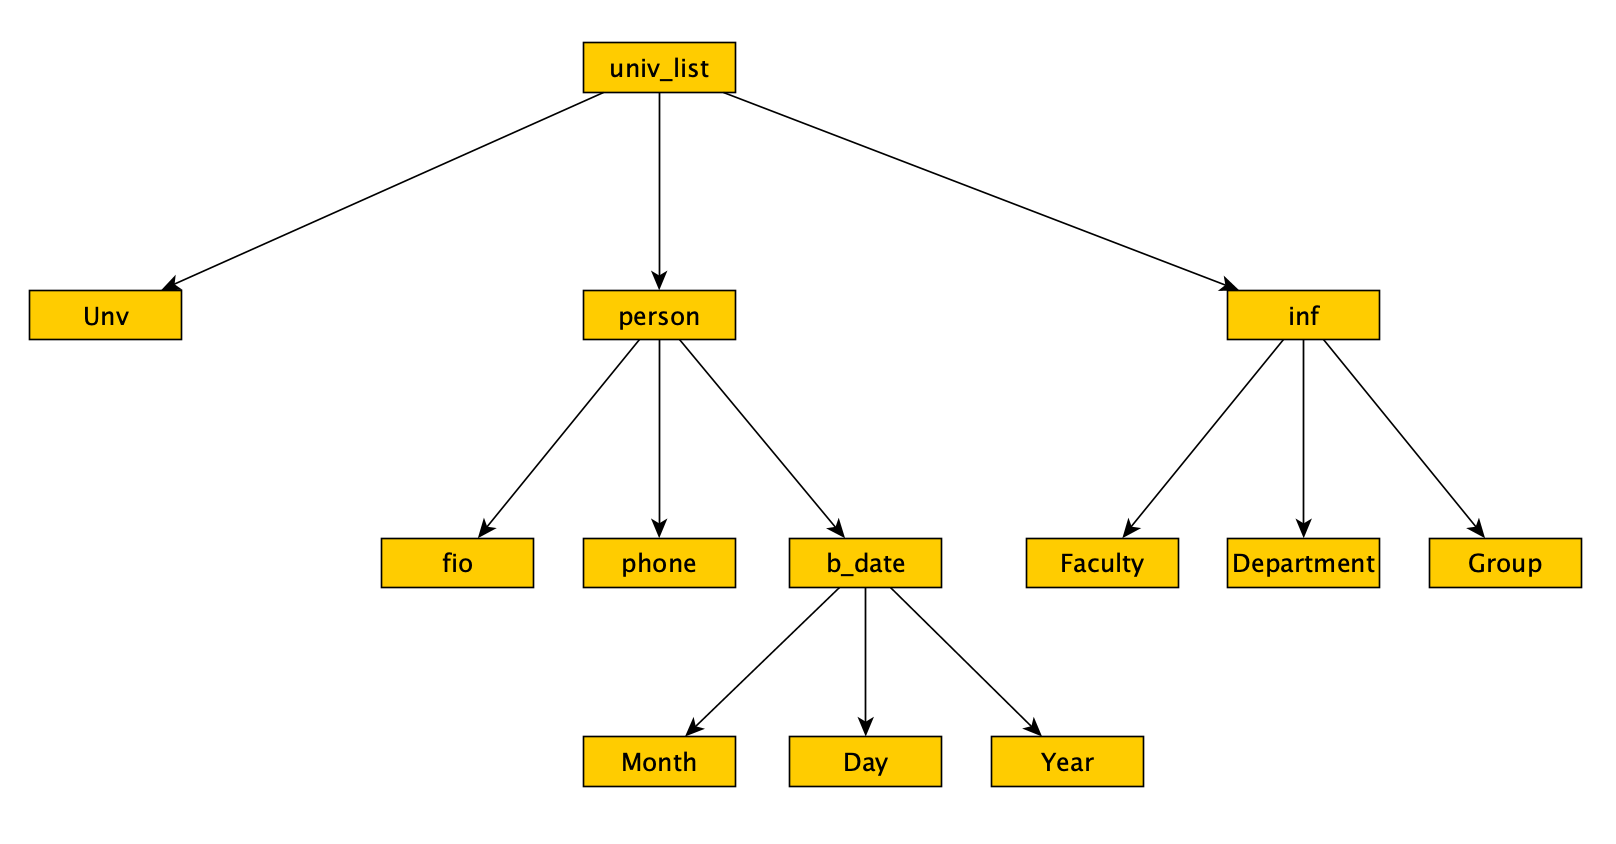
\includegraphics[scale = 0.6]{theme.png}}
		\end{center}
		\caption{Древовидная структура данных программы.}
		\label{ris:1}
	\end{figure}
	
	Данная база знаний формировалась с помощью фактов и правил. Правила использовались по аналогии с примером \textit{ch02e01.pro} из 11 лабораторной работы, чтобы присвоить одному терму те же параметры, что и другому (в данном случае присваивалась информация о факультете, кафедре и номере группы - \textit{inf(string Faculty, integer Department, integer Group)}, а также название университета - \textit{string Unv}).
	
	\section{Варианты вопросов и ответы на них в программе}
	
	Ниже приведены вопросы и ответы программы на них:
	
	\textit{Существуют ли люди, обучающиеся в МГУ (MSU)?}
	\begin{lstlisting}[label = lst_qw_1, caption = Пример 1]
	goal
		univ_list("MSU", Student, Info).
	Output:
		Student=person(name("Ilya","Levushkin"),"8-985-977-14-92",b_date("december",11,1999)), Info=inf("VMK",5,99)
		Student=person(name("Vova","Vova"),"8-985-977-14-00",b_date("may",13,2002)), Info=inf("VMK",5,99)
		Student=person(name("Roma","Romaich"),"8-985-977-14-01",b_date("may",12,2003)), Info=inf("VMK",5,99)
		Student=person(name("Roma","Roma"),"8-985-977-14-02",b_date("may",13,2003)), Info=inf("VMK",5,99)
		Student=person(name("Olya","Olyaich"),"8-985-977-14-03",b_date("may",12,2004)), Info=inf("VMK",5,99)
		Student=person(name("Olya","Olya"),"8-985-977-14-04",b_date("may",13,2004)), Info=inf("VMK",5,99)
		Student=person(name("Sveta","Svetaich"),"8-985-977-14-05",b_date("may",12,2005)), Info=inf("VMK",5,99)
		Student=person(name("Sveta","Sveta"),"8-985-977-14-06",b_date("may",13,2005)), Info=inf("VMK",5,99)
		8 Solutions
	\end{lstlisting}
	
	
	\textit{Существуют ли люди с именем Илья Левушкин (Ilya Levushkin)?}
	День рождения не интересует.
	\begin{lstlisting}[label = lst_qw_2, caption = Пример 2]
	goal
		univ_list(Unv, person(name("Ilya", "Levushkin"), Phone, _), Info).
	Output:
		Unv=Bauman, Phone=8-985-977-14-92, Info=inf("IU",7,62)
		Unv=MSU, Phone=8-985-977-14-92, Info=inf("VMK",5,99)
		2 Solutions
	\end{lstlisting}
	
	Поскольку Илья Левушкин обучается сразу в 2 ВУЗах найдено 2 решения.
	
	
	\textit{Есть ли в базе знаний студенты, учащиеся в Бауманском университете, на факультете ИУ, кафедры 6 и из группы 63? Вывести всех таких студентов.}
	\begin{lstlisting}[label = lst_qw_3, caption = Пример 3]
	goal
		univ_list("Bauman", Student, inf("IU", 6, 63)).
	Output:
		Student=person(name("Michel","Michel"),"433-9907",b_date("may",13,1982))
		Student=person(name("Dima","Dimaich"),"8-985-977-14-97",b_date("may",12,2001))
		Student=person(name("Dima","Dima"),"8-985-977-14-98",b_date("may",13,2001))
		Student=person(name("Vova","Vovaich"),"8-985-977-14-99",b_date("may",12,2002))
		4 Solutions
	\end{lstlisting}
	
	\textit{Есть ли в базе знаний студенты, учащиеся в МГУ 2003-ого года рождения? Вывести имена и номера телефонов этих студентов.}
	\begin{lstlisting}[label = lst_qw_4, caption = Пример 4]
	goal
		univ_list("MSU", person(Name, Phone, b_date(_, _, 2003)), _).
	Output:
		Name=name("Roma","Romaich"), Phone=8-985-977-14-01
		Name=name("Roma","Roma"), Phone=8-985-977-14-02
		2 Solutions
	\end{lstlisting}
	
	\section{Назначение и использование переменных}
	
	Ниже приведен список переменных с их описанием:
	\begin{itemize}
		\item \textit{Faculty (Номер факультета), Department (Номер кафедры), Group (Номер группы), Month (Месяц), Day (День), Year (год), First (Имя), Last (Фамилия), Phone (номер телефона)} - именованные переменные, связанные со стандартными доменами (\textit{string, integer}), не требующие описания;
		\item \textit{info (учебная информация о студенте)} - именованная переменная, связанная с составным доменом, образованным функтором \textit{inf} с параметрами \textit{string Faculty, integer Department, integer Group};
		\item \textit{birthday (день рождения)} - именованная переменная, связанная с составным доменом, образованным функтором \textit{b\_date} с параметрами \textit{string Month, integer Day, integer Year};
		\item \textit{fio (полное имя)} - именованная переменная, связанная с составным доменом, образованным функтором \textit{name} с параметрами \textit{string First, string Last};
		\item \textit{student (студент)} -  именованная переменная, связанная с составным доменом, образованным функтором \textit{person} с параметрами \textit{fio, string Phone, birthday}.
	\end{itemize}
	
	\section{Порядок формирования результата работы программы}
	Формирование результата происходит с помощью механизма унификации, встроенного в систему и не доступного программисту.
	
	Опишем процесс унификации для вопроса из примера 1 к нашей программе:
	
	Для Пролога вопрос есть цель, которую необходимо достичь. Пролог берет вопрос univ\_list(<<MSU>>, Student, Info) и начинает последовательно сверху-вниз сравнивать его с фактами и правилами базы знаний. Там где обнаруживается предикат с таким же идентификатором как и у вопроса и с таким же количеством аргументов происходит сопоставление.
	
	Так как в вопросе первый аргумент имеет конкретное значение, то Пролог проводит сопоставление сравнивая значение из вопроса и из фактов. Как только они совпадут, процесс сравнения переходит на вторые аргументы, третьи. В вопросе второй и третий аргументы ничем не обозначены, поэтому ему передаются значения из факта. О чем, собственно, Пролог и сообщает.

	
	\section{Ответы на вопросы}
	
	\subsection{Что собой представляет программа на Prolog?}
	
	Программа на Prolog представляет собой базу знаний и вопрос.
	
	\begin{itemize}
		\item База знаний состоит из предложений - CLAUSES (отдельных знаний или утверждений): фактов и правил.
		
		\item Вопрос состоит только из тела – составного терма (или нескольких составных термов). Вопросы используются для выяснения выполнимости некоторого отношения между описанными в программе объектами. Система рассматривает вопрос как цель, к которой (к истинности которой) надо стремиться.
	\end{itemize}
	
	\subsection{Какова структура программы на Prolog?}
	
	Программа на Prolog состоит из разделов. Каждый раздел начинается со своего заголовка. Структура программы:
	\begin{itemize}
		\item директивы компилятора — зарезервированные символьные константы
	    \item CONSTANTS — раздел описания констант
	    \item DOMAINS — раздел описания доменов
	    \item DATABASE — раздел описания предикатов внутренней базы данных
	    \item PREDICATES — раздел описания предикатов
	    \item CLAUSES — раздел описания предложений базы знаний
	    \item GOAL — раздел описания внутренней цели (вопроса).
	\end{itemize}
	В программе не обязательно должны быть все разделы.
	
	
	\subsection{Как программа реализуется на Prolog?}
	
	\begin{itemize}
		\item Предложения бывают двух видов: факты и правила;
		\item Каждое предложение заканчивается точкой;
		\item Предложение более общего вида – правило имеет вид:
$A :- B1,... , Bn$
		
		A называется заголовком правила, а B1,..., Bn – телом правила;
		\item Факт – это предложение, в котором отсутствует тело (частный случай правила);
	\end{itemize}
	
	
	\subsection{Как формируются результаты работы программы?}
	
	Ответ на поставленный вопрос система дает в логической форме – «Да» или «нет». Цель системы состоит в том, чтобы на поставленный вопрос найти возможность, исходя из базы знаний, ответить «Да». Вариантов ответить «Да» на поставленный вопрос может быть несколько. Система может (в нашем случае обучения - должна) быть  настроена в режим получения всех возможных вариантов ответа «Да» на поставленный вопрос.
	
	Поиск содержательного ответа на поставленный вопрос, с помощью имеющейся базы знаний, фактически заключается в поиске нужного знания, но какое знание понадобится – заранее неизвестно. Этот поиск осуществляется формально с помощью механизма \textit{унификации}, встроенного в систему и не доступного программисту. 
	
\end{document}